\documentclass[11pt]{article}

\usepackage{apacite}
\usepackage{amsmath,amssymb}
\usepackage{graphicx}
\usepackage{color}
\usepackage{url}
\usepackage[left=1in, right=1in, top=1in, bottom=1in]{geometry}
\usepackage{booktabs}

\newcommand{\tableref}[1]{Table \ref{#1}}
\newcommand{\figref}[1]{Figure \ref{#1}}
\newcommand{\sectionref}[1]{Section \ref{#1}}

\title{Reporting model results}

\author{Judith Degen}

\date\today

\begin{document}

\maketitle

\section{General notes on reporting results}

When reporting results, here's a good set of steps to follow:
\begin{enumerate}
	\item Start by pointing to a relevant visualization of the data and reminding the reader of the questions to be addressed with the data analysis. 
	\item Report the analysis you conducted (e.g., mixed effects logistic or linear regression) and the model specification: what was the outcome variable? What were the fixed and random effects? How were the fixed effects coded?
	\item Report the model coefficients and direction of effects.
	\item Optional: if you don't have a dedicated Discussion section, include brief discussion of results in the Results section.
\end{enumerate}

The next two sections contain examples of reporting mixed effects logistic regression (\sectionref{sec:logistic}) and mixed effects linear regression  (\sectionref{sec:linear}). The prose in \sectionref{sec:logistic} is taken (and slightly modified) from \citeA{DegenEtAl2020}. The prose in \sectionref{sec:linear} is taken (and slightly modified) from \citeA{DegenTonhauser-toappear}.

\newpage

\section{Example: reporting mixed effects logistic regression results}
\label{sec:logistic}

Proportions of redundant \emph{color-and-size} utterances are shown in \figref{fig:exp1results} alongside model predictions (to be explained further in Section 5. There are three main questions of interest: first, do we replicate the color/size asymmetry in probability of redundant adjective use? Second, do we replicate the previously established effect of increased redundant color use with increasing scene variation? Third, is there an effect of scene variation on redundant size use and if so, is it smaller compared to that on color use, as is predicted under asymmetric semantic values for color and size adjectives?

\begin{figure}[h]
\centering
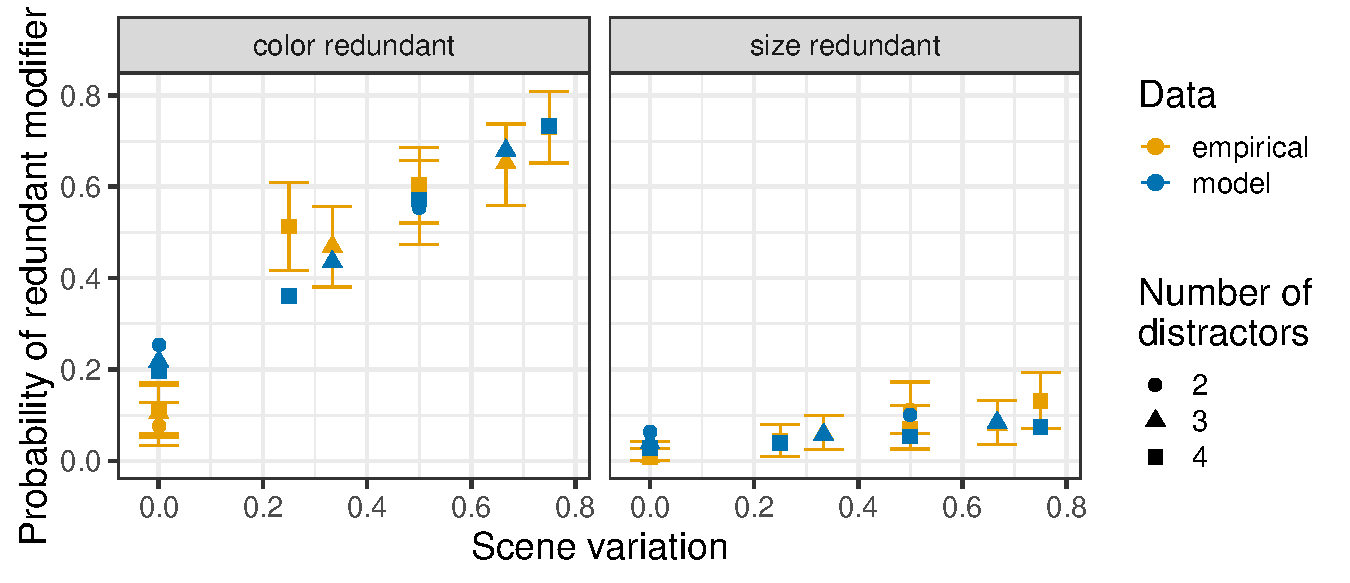
\includegraphics[width=.8\textwidth]{images/exp1-empirical-predictives}
\caption{Empirical redundant utterance proportions  (blue)  alongside point-wise maximum a posteriori (MAP) estimates of the RSA model's posterior predictives for redundant utterance probability (red) as a function of scene variation in the color redundant (left) and size redundant (right) condition. Here and in all following plots, error bars indicate 95\% bootstrapped confidence intervals.}
\label{fig:exp1results}
\end{figure}

We addressed all of these questions by conducting a single mixed effects logistic regression analysis predicting redundant over minimal adjective use from fixed effects of sufficient property (color vs.~size, centered, size positive), scene variation (proportion of distractors that does not share the insufficient property value with the target, centered), and the interaction between the two.\footnote{All mixed effects analyses reported in this paper were conducted with the \texttt{lme4} package \cite{lme4} in R \cite{R}.} The model included the maximal random effects structure justified by the design:\footnote{Alternatively: ``that allowed the model to converge"} by-participant and by-item random intercepts as well as by-participant random slopes for the fixed effects of sufficient property and scene variation.

We observed a main effect of sufficient property, such that speakers were more likely to redundantly use color than size adjectives ($\beta = 3.54$, $SE = .22$, $p < .0001$), replicating the much-documented color-size asymmetry. We further observed a main effect of scene variation, such that redundant adjective use increased with increasing scene variation ($\beta = 4.62$, $SE = .38$, $p < .0001$). Finally, we also observed a significant interaction between sufficient property and scene variation ($\beta = 2.26$, $SE = .74$, $p < .003$). Simple effects analysis revealed that the interaction was driven by the scene variation effect being smaller in the \emph{color-sufficient} condition ($\beta = 3.49$, $SE = .65$, $p < .0001$) than in the \emph{size-sufficient} condition ($\beta = 5.75$, $SE = .38$, $p < .0001$), as predicted if size modifiers are noisier than color modifiers. 

\section{Example: reporting mixed effects linear regression results}
\label{sec:linear}

Figure \ref{f-prior} shows the mean prior probabilities of the 20 contents by fact. To assess whether fact type affected prior content probability, we conducted a  mixed-effects linear regression predicting slider rating from dummy-coded fact type (reference level: `lower probability') and random by-item and by-participant intercepts and slopes for fact type.\footnote{All analyses were conducted in R \cite{R} using the \texttt{lme4} package \cite{lme4}.} Each content's mean prior probability  was rated as higher when it was presented with its higher probability fact than when it was presented with its lower probability fact ($\beta$ = 0.45, $SE$ = 0.01, $t$ = 31.12, $p$ $<$ .0001). This suggests that the manipulation of the prior probability of the 20 contents was successful. 

\begin{figure}[h!]
\centering
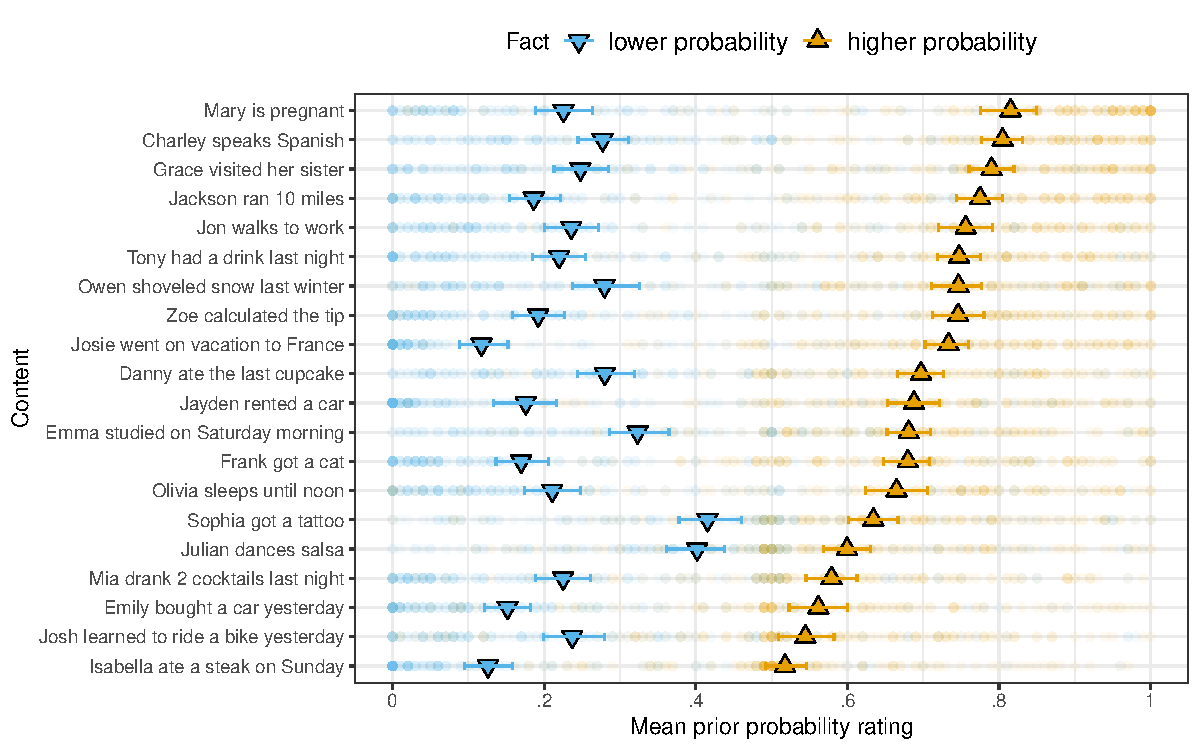
\includegraphics[width=.95\textwidth]{images/prior-ratings}

\caption{Mean prior probability by content and fact in Exp.~1. Error bars indicate 95\% bootstrapped confidence intervals. Transparent dots indicate individual participant ratings.} 
\label{f-prior}
\end{figure}

\bibliographystyle{apacite}

\setlength{\bibleftmargin}{.125in}
\setlength{\bibindent}{-\bibleftmargin}

\bibliography{bibs}


\end{document}
